% Chapter 6
\section[From estimation to inference]{From Estimation to Inference: Covariance, Precision, and Conditional Independence}\label{sec:ggm}

Chapter~\ref{sec:onedim} settled ``correlation $\neq$ causation'' in one dimension. This chapter upgrades the question to the joint level: treating $(y, \x)$ as a single $(d{+}1)$-dimensional random vector, we ask how the \textbf{covariance matrix and its inverse (the precision matrix)} encode the correlation, conditional independence, and — under graph assumptions — causal structure between $y$ and $\X$; and then we answer the practical questions: how to estimate when $d$ is large and $n$ is small (lasso, elastic net, CLIME, graphical lasso), and how to upgrade ``point estimation'' into ``inference'' (the debiased lasso) — in short, \textbf{from estimate to inference}.

\subsection{Covariance and Precision: Two Encodings of Correlation}\label{sec:cov-prec}

Let $(y, \x)$ be jointly Gaussian with mean zero (w.l.o.g.), and write
\[
  \bm{\Sigma} = \Cov\begin{pmatrix} y \\ \x \end{pmatrix} \succ \zero,
  \qquad
  \bm{\Theta} = \bm{\Sigma}^{-1} \ \text{(the precision matrix)}.
\]
The two matrices encode two different kinds of ``correlation'':

\begin{itemize}
  \item \textbf{$\Sigma_{ij} \neq 0$}: marginal correlation. It \textit{propagates}: even when $y \perp x_j$ given the remaining variables (no direct link), $x_j$ can remain marginally correlated with $y$ — as long as an indirect path through other variables exists (the multivariate version of the common-cause structure of Section~\ref{sec:1d-causality}).
  \item \textbf{$\Theta_{ij} = 0$}: \textbf{conditional independence}. In the Gaussian case there is an exact identity
  \begin{equation}\label{eq:ci-prec}
    \Theta_{ij} = 0
    \quad\Longleftrightarrow\quad
    i \perp j \mid \text{all remaining variables},
    \qquad
    \rho_{ij \cdot V \setminus \{i,j\}} = -\frac{\Theta_{ij}}{\sqrt{\Theta_{ii}\,\Theta_{jj}}} \, .
  \end{equation}
  The right-hand side is the \emph{partial correlation}: \textit{zero partial correlation $\Leftrightarrow$ independence given everything else.} The proof is just block inversion (Exercise~\ref{ex:block-inv}).
\end{itemize}

\eqref{eq:ci-prec} is the hinge of this chapter: \textbf{the zero pattern of the precision matrix is the adjacency matrix of a ``conditional-independence graph''} — the Gaussian graphical model\cite{lauritzen1996}. Correlation \textit{flows} along the graph (indirect paths create correlation); conditional independence holds exactly where there is \emph{no edge}. This graph is the Gaussian incarnation of Wright's path diagram (Section~\ref{sec:1d-causality}).

\subsection{Regression Coefficients Are Entries of the Precision Matrix}\label{sec:beta-theta}

Now plug linear regression into this picture. Block the joint Gaussian precision as $\bm{\Theta} = \begin{pmatrix} \Theta_{yy} & \bm{\Theta}_{yX} \\ \bm{\Theta}_{Xy} & \bm{\Theta}_{XX} \end{pmatrix}$ (scalar $\Theta_{yy} > 0$, $\bm{\Theta}_{Xy} \in \R^d$). By block inversion (Exercise~\ref{ex:block-inv}), the conditional distribution of $y$ given $\X$ is
\begin{equation}\label{eq:conditional}
  y \mid \X \sim \mathcal{N}\Big( -\tfrac{1}{\Theta_{yy}}\, \bm{\Theta}_{yX}^\top \x,\ \tfrac{1}{\Theta_{yy}} \Big).
\end{equation}
Comparing with the regression model $y = \x^\top \bbeta + \varepsilon$ yields a set of identities that deserve to be carved in stone:
\begin{equation}\label{eq:beta-theta}
  \boxed{\;\bbeta = -\frac{\bm{\Theta}_{Xy}}{\Theta_{yy}}, \qquad \Var(\varepsilon) = \frac{1}{\Theta_{yy}}\;}
\end{equation}

\begin{keybox}[Regression $=$ probing the graph]
\eqref{eq:beta-theta} says: \textbf{regression coefficients (together with their signs and significance) are ratios of precision-matrix entries.} In particular,
\[
  \beta_j = 0
  \quad\Longleftrightarrow\quad
  \Theta_{Xy,j} = 0
  \quad\Longleftrightarrow\quad
  y \perp x_j \mid \x_{-j} .
\]
i.e., $y$ and $x_j$ are independent given all the other features.
\end{keybox}

This sentence translates one statistical problem into two:
\begin{enumerate}[label=(\arabic*)]
  \item \textbf{Correlation} (Chapter~\ref{sec:onedim}): are $y$ and $x_j$ marginally correlated? — read off $\bm{\Sigma}$, one $t$-test;
  \item \textbf{Conditional independence}: controlling for everything else, is there still a ``direct'' link between $y$ and $x_j$? — read off the zero pattern of $\bm{\Theta}$, i.e.\ whether the \textbf{partial correlation} is zero.
\end{enumerate}
The gap between the two is the matrix language of phenomena like ``the correlation between $x_j$ and $y$ is entirely explained by a third variable'' (confounding, mediation). Note that $\beta_j = 0$ delivers a \textbf{graph-theoretic ``no direct edge''}, not a causal claim — unless the graph itself has already been pinned down as identifiable by external knowledge (Section~\ref{sec:1d-causality}) or by the conditional-independence tests below.

\subsection{Conditional-Independence Testing and Causality: From Correlation to Graph}\label{sec:ci-causal}

\eqref{eq:ci-prec} supplies \textbf{testable constraints}: every missing edge on a Gaussian graph corresponds to a statistical hypothesis of zero partial correlation
\begin{equation}\label{eq:ci-test}
  H_0^{(ij)}:\ \rho_{ij\cdot V\setminus\{i,j\}} = 0
  \quad(\Longleftrightarrow\ \Theta_{ij} = 0),
\end{equation}
which Fisher's $z$-transform can test directly in low dimensions; in high dimensions individual testing becomes infeasible, but the logic of the constraints is unchanged. The PC algorithm (Spirtes, Glymour \& Scheines) shows how such constraints turn into causal discovery\cite{spirtes2000}:

\begin{enumerate}[label=(\alph*)]
  \item \textbf{Edge deletion}: for each pair of variables, search over conditioning sets $S$; as soon as $i \perp j \mid S$ is accepted, delete the undirected edge between $i$ and $j$ — common causes and indirect paths are exposed by exactly this test (the operable version of Reichenbach's principle\cite{reichenbach1956});
  \item \textbf{Orientation}: for structures $i - k - j$ with $i, j$ nonadjacent (v-structures), Markov $+$ faithfulness allow orienting $i \to k \leftarrow j$ — \textbf{the data itself gives the direction of some arrows};
  \item \textbf{Propagation}: Meek's rules propagate orientations further along the graph.
\end{enumerate}

Echoing Chapter~\ref{sec:onedim}: the correlation coefficient never yields direction, but \textbf{a battery of conditional-independence tests} can recover part of the DAG under the additional assumption that the distribution is faithful to a graph; the validity of causal conclusions still comes from the assumption list, not from the data itself — except that now each assumption can be tested and refuted one by one.

\subsection{Sparsity: Why ``Most Coefficients Are Zero'' Is a Computable Assumption}\label{sec:sparsity}

The preceding sections gave the language of graphical models: up to $\binom{d}{2}$ edges among $d$ variables, $d^2$ precision-matrix entries to estimate. When $d > n$ this is hopeless — unless we are willing to believe something very specific: \textbf{the true graph is sparse}, and most $\Theta_{ij} = 0$. This section explains why the assumption is not only plausible but ``computable.''

\textbf{Sparsity is a falsifiable assumption, not a prayer.} ``Most coefficients are zero'' means the graph has $s \ll d^2$ edges; when the true edge count satisfies $s \log d \ll n$, a family of methods (next section) recovers the graph structure \textbf{exactly} with high probability. Conversely, if the world is truly dense, sparse methods fail honestly — cross-validation will not settle on a stable structure. This matches the Chapter~\ref{sec:1d-causality} spirit of ``fit first, then audit the assumptions'': the sparsity assumption can and should be audited.

\textbf{Where does sparsity come from?} Three independent sources. (1) \textbf{Scientific}: in gene regulatory networks each gene is regulated by few transcription factors; in social networks each person has few close contacts — ``bounded nonzeros per row'' is prior knowledge in many fields, mathematically $s = O(d)$ edges. (2) \textbf{Statistical}: under suitable designs, a sparse model's effective degrees of freedom are $\ll d$ (below), and the sample complexity is governed by the \textbf{number of nonzeros} rather than the dimension — this is the very meaning of the term ``high-dimensional statistics'': $d$ may exceed $n$ as long as the support of the true parameter is smaller than $n$. (3) \textbf{Computational}: sparsity turns a $d^2$-dimensional continuous optimization into ``find which coordinates are nonzero $+$ estimate their values,'' and the latter has explicit algorithms and error bounds.

\textbf{Three faces of sparsity, one sentence each.}
\begin{enumerate}[label=(\arabic*)]
  \item \textbf{Combinatorial face}: model selection — finding the correct one among $2^d$ subsets. The general problem is NP-hard, but under sparsity it becomes tractable (small $s$ collapses the search space).
  \item \textbf{Geometric face}: the $\ell_0$ ball $\{\bbeta : \norm{\bbeta}_0 \le s\}$ is nonconvex, but its \textbf{convex hull} is the $\ell_1$ ball $\{\bbeta : \norm{\bbeta}_1 \le R\}$ — $\ell_1$ is the ``convex relaxation'': the relaxed problem is convex again, and the price of relaxation (recovery conditions) can be quantified via incoherence and the restricted eigenvalue condition.
  \item \textbf{Statistical face}: effective degrees of freedom --- the lasso fit $\X\widehat{\bbeta}$ has $\widehat{df} = \E[\norm{\widehat{\bbeta}}_0]$, so \textbf{a sparse model's complexity is charged by the variables it actually uses}, not by $d$. This explains why the variance of a sparse estimator can be far below $O(d/n)$.
\end{enumerate}

\textbf{An honest caveat}: sparsity is an \textbf{assumption about the world}, not a mathematical trick. If the true signal is dense but decaying (e.g.\ $\beta_j \propto 1/j$), strongly sparse methods will systematically miss weak signals — ridge (dense shrinkage) may then be the more honest choice. Choosing lasso over ridge is choosing which world you believe; the bias--variance language of Section~\ref{sec:hd-break} quantifies the trade-off.

With these three faces in hand, the next section turns to concrete methods of estimation: lasso, elastic net, graphical lasso, and CLIME — four methods, all nailing the assumption ``sparse'' into an estimator through different optimization forms.

\subsection{Estimation: Four Regularizations for Large $d$, Small $n$}\label{sec:ggm-estimate}

The sample covariance $\bm{S} = \frac{1}{n}\X^\top\X$ (after centering) is singular when $d > n$; $\bm{S}^{-1}$ does not exist — \textbf{without regularization there is no precision matrix}. Four approaches, one goal (sparse $\bm{\Theta}$):

The first two act directly on regression coefficients. The lasso (Tibshirani, 1996) solves
\begin{equation}\label{eq:lasso}
  \min_{\bbeta} \ \frac{1}{2n} \norm{\y - \X \bbeta}^2 + \lambda \norm{\bbeta}_1 ,
  \qquad
  \norm{\bbeta}_1 = \sum_{j=1}^d |\beta_j| ,
\end{equation}
whose $\ell_1$ geometry (the corners of the constraint set) drives some coordinates \textbf{exactly} to $0$, yielding sparse solutions. Elastic net (Zou \& Hastie, 2005) combines $\ell_1$ with $\ell_2$:
\begin{equation}\label{eq:enet}
  \min_{\bbeta} \ \frac{1}{2n} \norm{\y - \X \bbeta}^2 + \lambda \Big( \alpha \norm{\bbeta}_1 + \tfrac{1-\alpha}{2} \norm{\bbeta}^2 \Big),
\end{equation}
where the $\ell_2$ term lets \textbf{whole groups of highly correlated variables enter the model together} (fixing lasso's habit of picking one member of a correlated group at random) — well suited to group-correlated data such as gene expression. The remaining two move the penalty to the matrix level:

\begin{itemize}
  \item \textbf{Nodewise lasso} (Meinshausen \& Bühlmann, 2006): regress each variable on all the others via \eqref{eq:lasso}, and connect $i$ to $j$ in the graph whenever a coefficient is nonzero — Section~\ref{sec:beta-theta} says this is equivalent to recovering the precision matrix column by column\cite{tibshirani1996,meinshausen2006}.
  \item \textbf{Graphical lasso} (Friedman, Hastie \& Tibshirani, 2008): penalize the likelihood of the precision matrix directly,
  \[
    \min_{\bm{\Theta} \succ \zero} \ \trace(\bm{S}\bm{\Theta}) - \log\det \bm{\Theta} + \lambda \norm{\bm{\Theta}}_1 ,
  \]
  estimating the whole graph in one shot; its optimality condition $\bm{S} - \bm{\Theta}^{-1} + \lambda \bm{\Gamma} = \zero$ ($\bm{\Gamma}$ a subgradient) hooks estimation directly to conditional-independence testing\cite{friedman2008}.
  \item \textbf{CLIME} (Cai, Liu \& Luo, 2011): leave the likelihood alone and solve
  \[
    \min_{\bm{\Theta}} \ \norm{\bm{\Theta}}_1 \quad \text{s.t.} \quad \norm{ \bm{S}\bm{\Theta} - \bm{I} }_{\max} \le \lambda ,
  \]
  i.e.\ ``find a sparse matrix that is approximately the inverse of $\bm{S}$.'' It is a \textbf{linear program} (column by column), needs no $\bm{\Theta} \succ \zero$ constraint and no $\log\det$ computation, gives spectral-norm convergence rates under weaker assumptions, and natively fits scenarios where ``$\bm{\Sigma}$ need not be sparse, only $\bm{\Theta}$ is''\cite{cai2011}.
\end{itemize}

What the four share is the bias--variance trade (Section~\ref{sec:hd-break}) replayed at the matrix level: $\lambda$ crushes masses of $\Theta_{ij}$ to $0$, trading a little bias for a controlled variance of the covariance inversion. Figure~\ref{fig:ch6-lassopath} plots the regularization path of \eqref{eq:lasso} — its solution as a function of $\lambda$.

\begin{figure}[htbp]
  \centering
  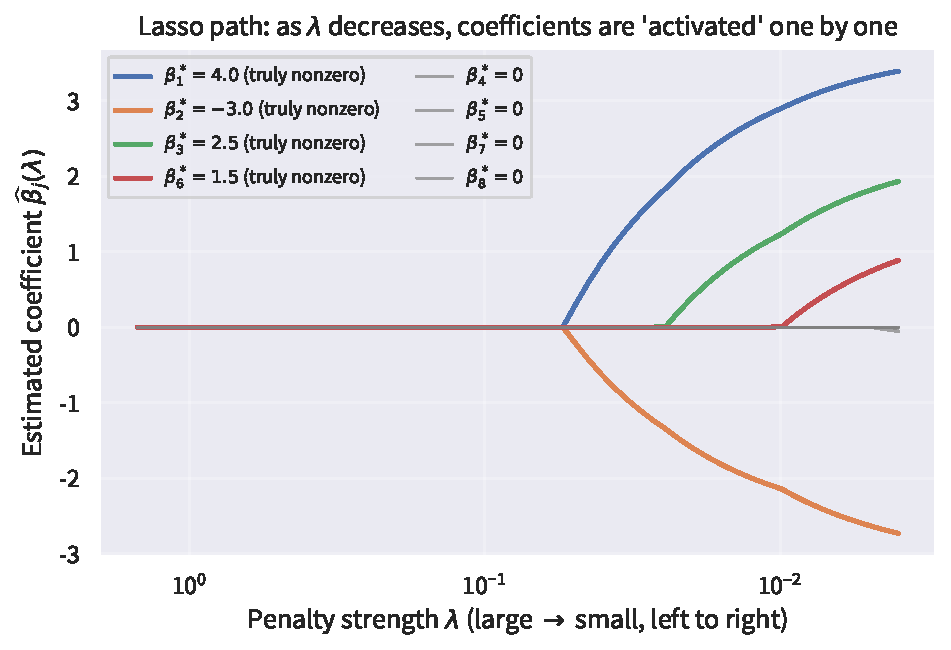
\includegraphics[width=0.85\linewidth]{figures/ch6_lassopath.pdf}
  \caption{The lasso regularization path (simulated data, true coefficients $4,-3,2.5,0,0,1.5,0,0$): as $\lambda$ decreases (horizontal axis, large on the left), the four truly nonzero coefficients (colored) are ``activated'' one by one from $0$, while the truly zero coefficients (gray) stay pinned at $0$ — sparsity is not assumed but selected automatically by the geometry (diamond-shaped constraint corners) of the $\ell_1$ penalty.}
  \label{fig:ch6-lassopath}
\end{figure}

\subsection{Inference: The Debiased Lasso and Tests of Conditional Independence}\label{sec:debiased}

Once the estimate $\hat\beta_j$ is in hand, a \textbf{point estimate cannot be turned into a $p$-value directly}: the lasso's shrinkage biases $\hat\beta_j$, and its limiting distribution is not Gaussian. The way out is \textbf{debiasing} (debiasing / desparsifying). The idea in one sentence: \textit{add back what the penalty stole}. Take a nodewise estimate $\widehat{\bm{\Theta}}$ of the precision matrix (e.g.\ nodewise lasso regressions of $\bm{S}$, or CLIME directly), and define
\begin{equation}\label{eq:debiased}
  \widetilde{\bbeta} = \widehat{\bbeta}_{\mathrm{lasso}} + \tfrac{1}{n}\, \widehat{\bm{\Theta}}\, \X^\top \big( \y - \X \widehat{\bbeta}_{\mathrm{lasso}} \big).
\end{equation}
Algebraically (Exercise~\ref{ex:debiased}): $\widetilde{\bbeta} - \bbeta = \frac{1}{n}\widehat{\bm{\Theta}}\X^\top \bm{\varepsilon} + (\bm{I} - \widehat{\bm{\Theta}}\bm{S})(\bbeta - \widehat{\bbeta}_{\mathrm{lasso}})$ — the first term is noise (asymptotically normal), the second a residual bias ($o_p(n^{-1/2})$ under sparsity). Hence (Zhang \& Zhang, 2014; van de Geer et al., 2014)
\begin{equation}\label{eq:asym-norm}
  \sqrt{n}\, \big( \widetilde{\beta}_j - \beta_j \big) \ \xrightarrow{d}\ \mathcal{N}\Big( 0,\ \sigma^2 \big( \bm{\Theta}\, \bm{\Sigma}\, \bm{\Theta} \big)_{jj} \Big),
  \qquad
  \text{confidence intervals:}\ \widetilde{\beta}_j \pm z_{1-\alpha/2}\, \frac{\hat\sigma}{\sqrt{n}} \sqrt{ \big( \widehat{\bm{\Theta}}\, \bm{S}\, \widehat{\bm{\Theta}} \big)_{jj} } .
\end{equation}
\cite{zhang2014,vandegeer2014} In high dimensions, \textbf{asymptotically normal inference for a single coefficient} is thus restored — and by \eqref{eq:beta-theta}, testing $H_0: \beta_j = 0$ \emph{is} \textbf{testing the conditional independence of $y$ and $x_j$}. The whole pipeline closes:

\begin{keybox}[From estimate to inference]
\[
\begin{gathered}
\underbrace{\text{lasso / elastic net / CLIME / glasso estimate }\bm{\Theta},\bbeta}_{\text{Section~\ref{sec:ggm-estimate}: sparse point estimation (biased, fast)}}
\\[1.2ex]
\Big\downarrow
\\[0.6ex]
\underbrace{\text{debias: }\widetilde{\bbeta} = \widehat{\bbeta} + \tfrac1n\widehat{\bm{\Theta}}\X^\top(\y - \X\widehat{\bbeta})}_{\text{add back what the penalty stole}}
\\[1.2ex]
\Big\downarrow
\\[0.6ex]
\underbrace{\text{asymptotic normality \eqref{eq:asym-norm} $\Rightarrow$ confidence intervals / } H_0:\beta_j=0 \Leftrightarrow y \perp x_j \mid \x_{-j}}_{\text{conditional-independence tests, and (under graph assumptions) a causal reading}}
\end{gathered}
\]
Estimation answers ``which edges might exist''; inference answers ``whether this edge is too significant to be noise''; between the two stands one debiasing step — the standard path by which high-dimensional statistics walks from ``prediction'' to ``scientific assertion.''
\end{keybox}

\textit{Single}-coefficient $p$-values aside, the working applied scientist faces an entire page of simultaneously tested conclusions — ``how many of these are real'' becomes the new question. Multiple-testing control of the false discovery rate (the BH procedure, knockoffs) is the subject of Chapter~\ref{sec:fdr}, and the closing of the loop of the sparsity story on the testing side.

\begin{exercise}\label{ex:block-inv}
Block inversion: for $\bm{\Sigma} = \begin{pmatrix} \Sigma_{yy} & \bm{\Sigma}_{yX} \\ \bm{\Sigma}_{Xy} & \bm{\Sigma}_{XX} \end{pmatrix}$ with inverse $\bm{\Theta} = \bm{\Sigma}^{-1}$, verify \eqref{eq:conditional} and \eqref{eq:beta-theta} from the blocks of $\bm{\Theta}$, and derive the partial-correlation formula \eqref{eq:ci-prec}.
\end{exercise}

\begin{exercise}\label{ex:debiased}
Derive the error decomposition $\widetilde{\bbeta} - \bbeta = \frac{1}{n}\widehat{\bm{\Theta}}\X^\top\bm{\varepsilon} + (\bm{I} - \widehat{\bm{\Theta}}\bm{S})(\bbeta - \widehat{\bbeta}_{\mathrm{lasso}})$ for \eqref{eq:debiased}, and explain why the two terms are, respectively, ``variance'' and ``bias.''
\end{exercise}

\begin{exercise}\label{ex:glasso-clime}
Compare the optimality conditions of graphical lasso and CLIME: the former writes ``$\bm{\Theta}$ is the inverse of $\bm{S}$'' as $\bm{S} - \bm{\Theta}^{-1} + \lambda\bm{\Gamma} = \zero$ (depending on $\bm{\Theta}$ being positive definite and invertible), the latter as $\bm{S}\bm{\Theta} - \bm{I} \approx \zero$ (linear constraints). Discuss: when $d \gg n$ and $\bm{S}$ is severely ill-conditioned, which optimization problem is better posed? What practical advantages does CLIME's column-by-column LP structure bring?
\end{exercise}
